\documentclass[10pt]{book}
\usepackage{commands}

\usepackage{bbm}


\begin{document}




\begin{tikzpicture}[remember picture,overlay]
	% If a chapter image has been specified
	\expandafter\ifstrequal\expandafter{\thechapterimage}{}{}{
		% Output the chapter image
		\node[
		anchor=north west, % Anchor point on the image
		inner sep=0pt, % Inner padding
		] at (current page.north west) {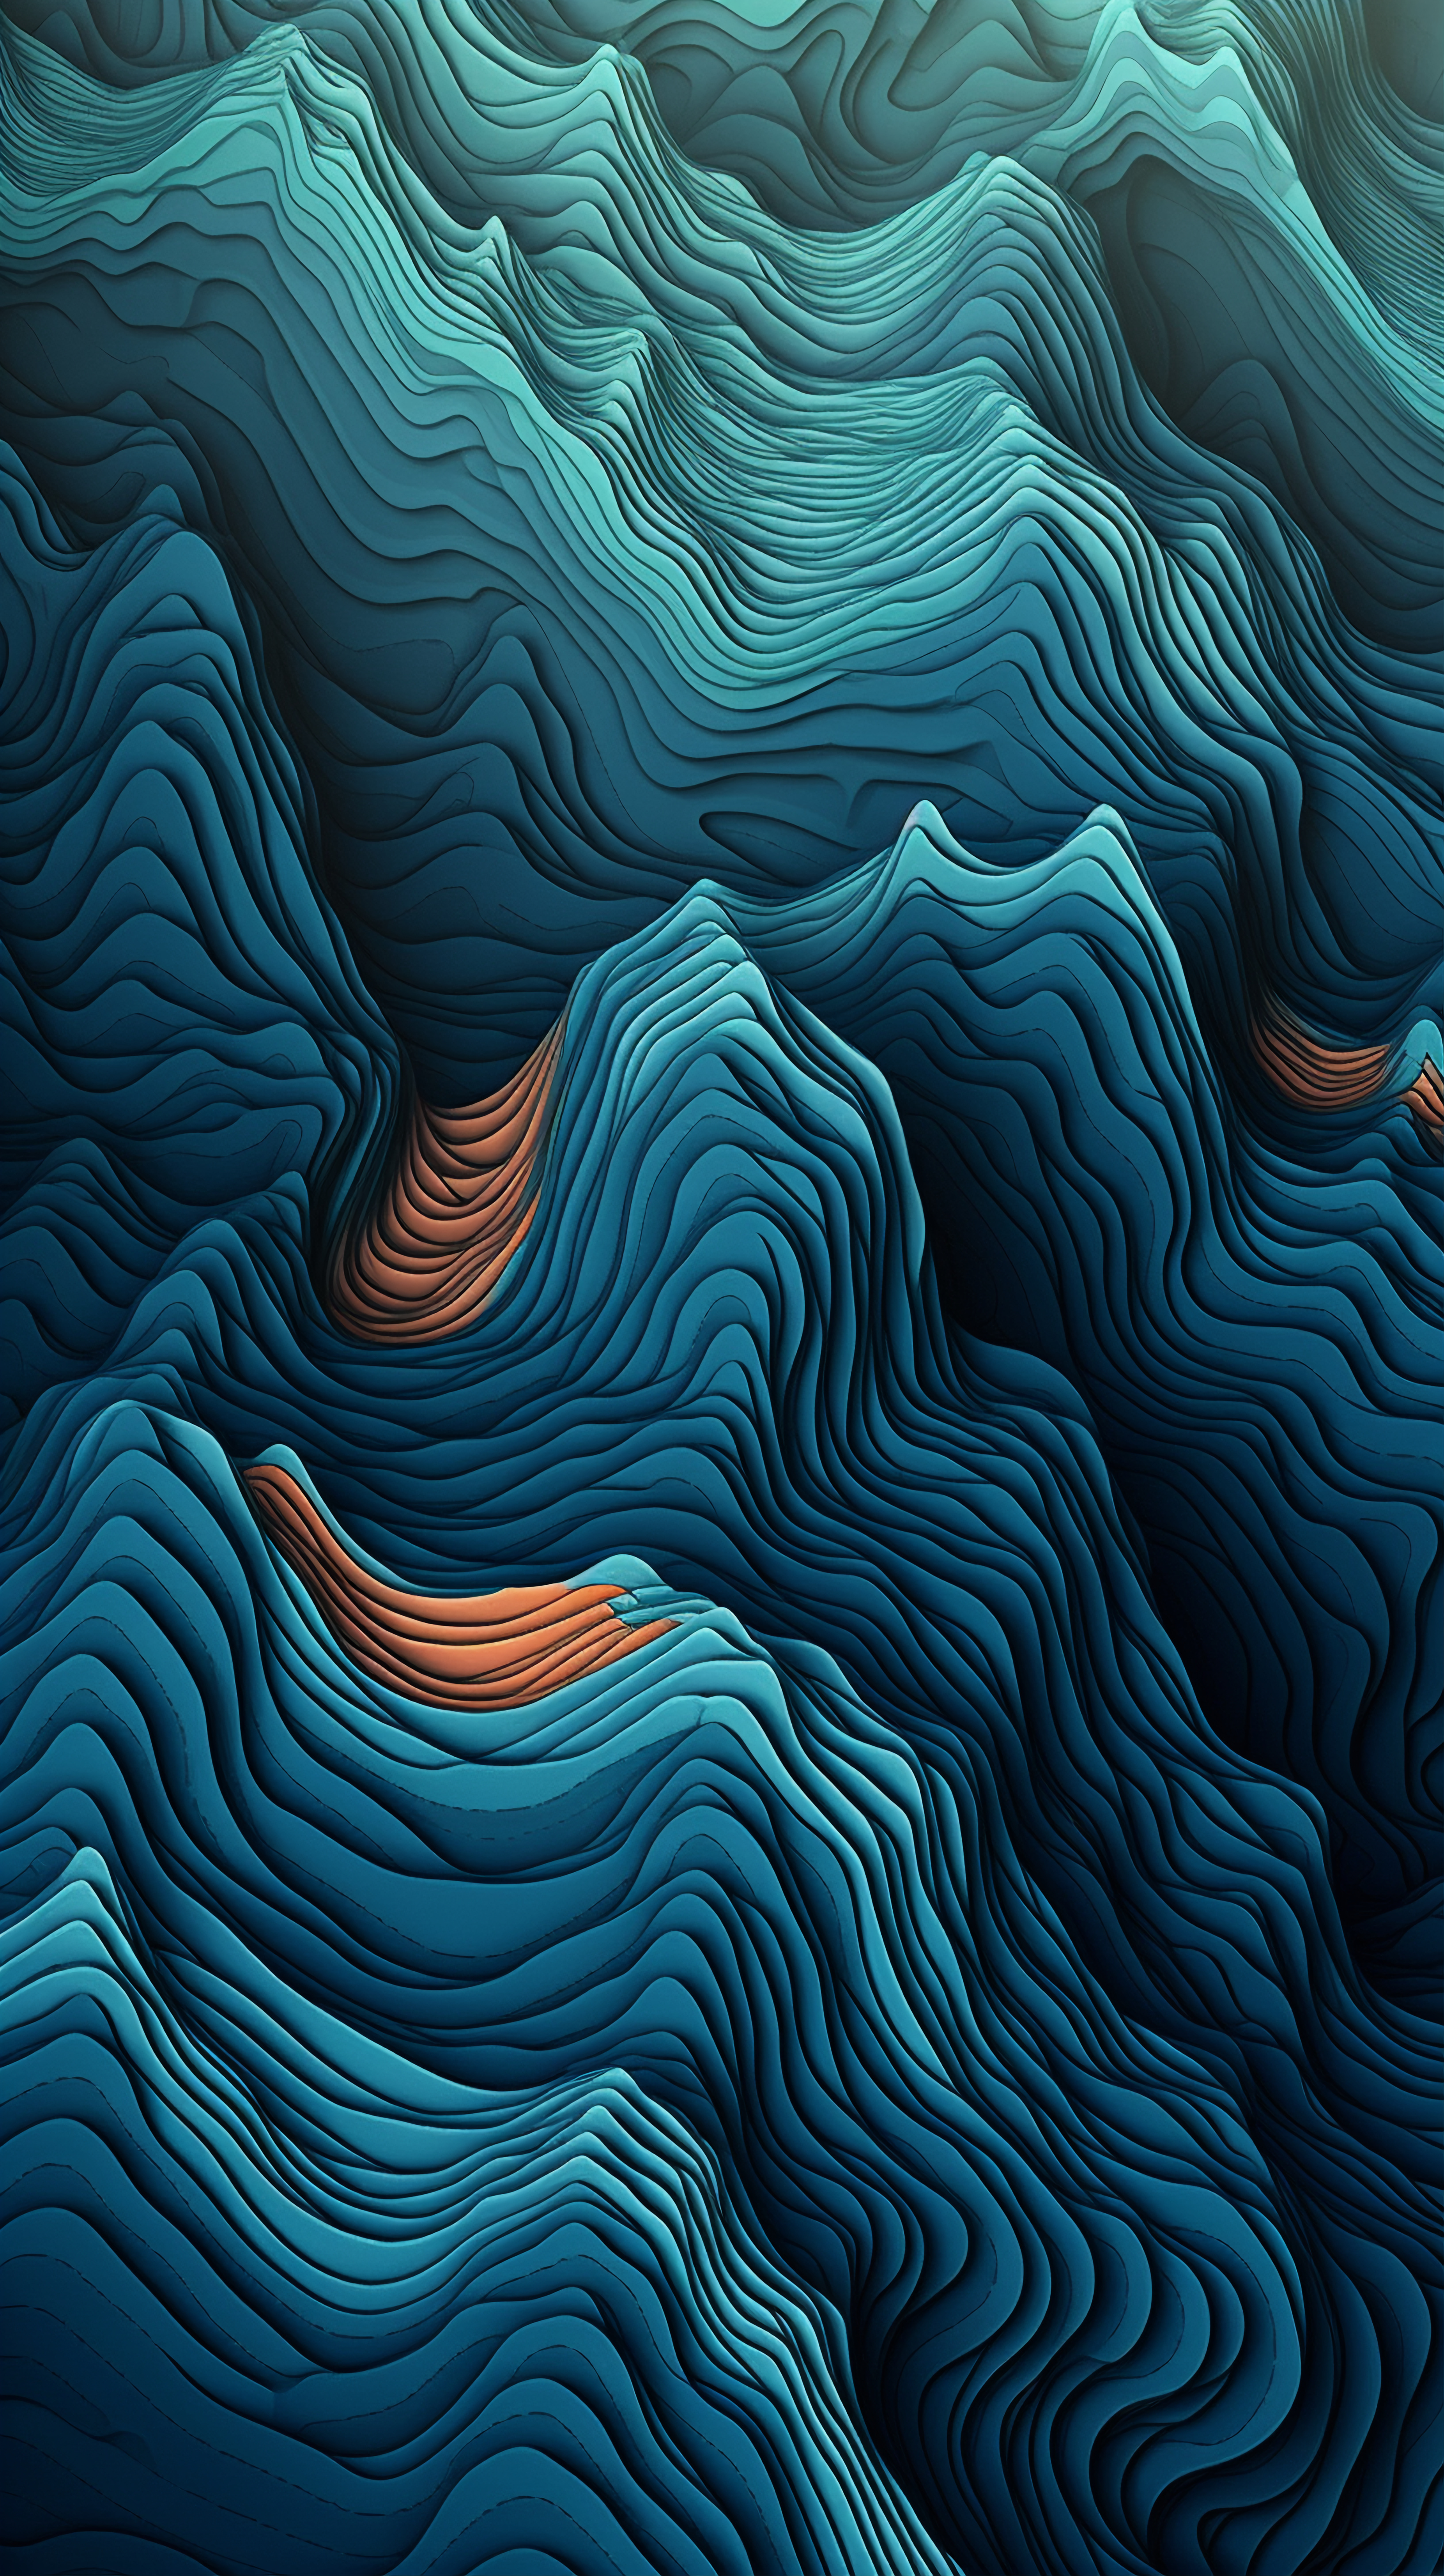
\includegraphics[angle=0,width=\paperwidth]{Images/output}};
	}
\end{tikzpicture}

\vspace{7cm}

\heading{Topology}


%\begin{figure}[h!]
%	\centering
%	\includegraphics[width=1\linewidth]{Images/realAnalysis}
%	\caption*{$\mathbb{R}$eal Analysis, Created by DALL-E!}
%	\label{fig:realanalysis}
%	
%\end{figure}




\tableofcontents

\chapter{Topological Spaces and Continuous Function}

\begin{definition}[Topology on a set]
	Let $ X $ be a set. A topology on $ X $ is a collection of subsets of $ X $, called \emph{open sets} and denoted by $ \mathcal{T} $, that satisfies
	\begin{itemize}[noitemsep]
		\item $ X,\emptyset \in \mathcal{T} $,
		\item For an \emph{arbitrary} collection of open sets $ \set{U_\alpha}_{\alpha \in J} $ we have
		\[ \bigcup_{\alpha\in J} U_\alpha \in \mathcal{T}. \]
		\item For a \emph{finite} collection of open sets $ \set{U_1,\cdots,U_n} $ for some $ n\in \N $ we have
		\[ \bigcap_{i=1}^n U_i \in \mathcal{T} \]
	\end{itemize}
\end{definition}

\begin{definition}[Finer and Coarse Topologies]
	\label{def:finer_and_coarse_topol}
	Let $ X $ be a set and $ \mathcal{T}_1 $ and $ \mathcal{T}_2 $ two topologies. The we say the topology $ \mathcal{T}_1 $ is finer if we have $ \mathcal{T_2} \subset \mathcal{T_1} $. Or alternatively, we can call the topology $ \mathcal{T}_2 $ to be coarser.
\end{definition}

\begin{definition}[Bases for a topology]
	Let $ X $ be a set. A collection of subsets of $ X $, denoted by $ \mathbb{B} $, is called a basis for the topology on $ X $ if we have
	\begin{itemize}[noitemsep]
		\item $ \forall x \in X $ there exists $ B \in \mathbb{B} $ such that $ x \in B $.
		\item If for sets $ B_1,B_2 \in \mathbb{B} $ we have $ x \in B_1\cap B_2 $, then $ \exists B_3 \in \mathbb{B} $ such that $ x \in B_3 \subset B_1\cap B_2 $.
	\end{itemize}
\end{definition}

\begin{definition}[Topology Generated by a Basis]
	\label{def:topology_generated_by_a_basis}
	Let $ X $ be a set and $ \mathbb{B} $ a basis for a topology. We \emph{define the topology $ \mathcal{T} $ generated by $ \mathbb{B} $} as follow: For any $ U \in \mathcal{T} $ and $ x \in U $ there exists $ B \in \mathcal{B} $ such that $ x \in B \subset U $.
\end{definition}
\begin{remark}
	\label{remark:TopologyGeneratedByABasis}
	We can now check that if $ \mathcal{T} $ generated by $ \mathbb{B} $ is really a topology. We need to show that $ \mathcal{T} $ has the topology properties.
	\begin{itemize}
		\item The statement $ \emptyset \in \mathcal{T} $ is vacuously true. To see $ X \in \mathcal{T} $, Consider $ x \in X $. Then from the definition of a basis $ \exists B \in \mathbb{B} $ such that $ x \in B $ and since $ X $ is the whole space, thus $ x \in B \subset X $.
		\item Let $ \set{U_\alpha}_{\alpha \in J} $ be an arbitrary collection of sets in $ \mathcal{T} $. Consider $ x \in \bigcup_\alpha U_\alpha $. Then there exists an index $ \alpha $ such that $ x \in U_\alpha $. Since $ U_\alpha \in \mathcal{T} $ thus there exists $ B \in \mathbb{B} $ such that $ x \in B \subset U_\alpha $ which implies $ x \in B \subset \bigcup_\alpha U_\alpha $, hence $ \bigcup_\alpha U_\alpha \in \mathcal{T} $.
		\item To see that the intersection of a finite collection of sets in $ \mathcal{T} $ is also in $ \mathcal{T} $, first if $ U_1 \in \mathcal{T} $ and $ U_2 \in \mathcal{T} $, then $ U_1 \cap U_2 \in \mathcal{T} $. That is because for $ x\in U_1 \cap U_2 $ we know that $ \exists B_1,B_2 \in \mathbb{B} $ such that $ x\in B_1\cap B_2 $. Thus from the definition of a basis $ \exists B_3 \in \mathbb{B} $ such that $ x \in B_3 \subset B_1\cap B_2 \subset U_1\cap U_2 $, hence $ U_1\cap U_2 \in \mathcal{T} $. Then by induction we can conclude that for any finite collection of sets in $ \mathcal{T} $ their intersection is also in $ \mathcal{T} $.
 	\end{itemize}
\end{remark}

\begin{proposition}[Characterization of Open Sets in Terms of Basis]
	\label{prop:charac_open_sets_in_terms_of_basis}
	Let $ X $ be a set and $ \mathbb{B} $ a basis for a topology $ \mathcal{T} $ on $ X $. Then $ \mathcal{T} $ is the collection of all unions of $ \mathbb{B} $.
\end{proposition}
\begin{proof}
	Let $ \mathcal{A} $ be the collection of all unions of $ \mathbb{B} $. We need to show the equality of the sets  
	\[ \mathcal{A} = \mathcal{T}. \]
	Let $ A \in \mathcal{A} $. Thus $ A = \bigcup_\alpha B_\alpha $ for $ B_\alpha \in \mathbb{B} $. Let $  x \in A $. Then we can choose any $ B_\alpha $ and we will have $ x \in B_\alpha \subset A $. Thus $ A \in \mathcal{T} $. To show the converse let $ A \in \mathcal{T} $. Thus for any $ x\in A $ we have $ B_x \in \mathbb{B} $ such that $ x \in B_x \subset A $. We can write
	\[ A = \bigcup_{x \in A} B_x. \]
	Thus $ A \in \mathcal{A} $. This completes the proof.
\end{proof}


\begin{carefull}[Be Aware of the Terminology]
	From the proposition above, we can say that a subset $ U \subset X $ is open (i.e. $ U \in \mathcal{T} $) if it can be written as union of sets in $ \mathbb{B} $. This union, however, need not be unique. This is a very important difference with the notion of basis in linear algebra, where given a basis for a space, we can then write any vector in the space uniquely by the basis vectors.
\end{carefull}


\begin{proposition}[Basis of a Given Topology]
	Let $ (X,\mathcal{T}) $ be a given topological spaces. A collection of open sets $ \mathcal{C} $ is a basis for the topology if $ \forall U \in \mathcal{T} $ and $ x \in U $ there exists $ C \in \mathcal{C} $ such that $ x\in C \subset U $.
\end{proposition}

\begin{proof}
	This proof has two steps. First, we need to show that the collection $ \mathcal{C} $ is indeed a basis, and then we need to show that the topology that this basis generates is the same as the topology of the set itself.
	
	\noindent \textbf{Showing that $ \mathcal{C} $ is a basis}. To show the first property of being a basis, we need to show that $ \forall x \in X $ we can find an element of $ \mathcal{C} $ that contains $ x $. Since $ X \in \mathcal{T} $ and by hypothesis we can find  $ C \in \mathcal{C} $ such that $ x \in C \subset X $, thus $ \mathcal{C} $ has the first property of being a basis. For the second property, we need to show that if $ x \in C_1 \cap C_2 $ then there exists $ C_3 \in \mathcal{C} $ such that $ x \in C_3 \subset C_1\cap C_2 $. Let $ x\in C_1\cap C_2 $ for $  C_1 , C_2 \in \mathcal{C} $. Since $ C_1,C_2 $ are open sets, then $ C_1\cap C_2 $ is also open. Thus by hypothesis there exists $ C \in \mathcal{C} $ such that $ x \in C \subset C_1\cap C_2 $. This completes the proof that the collection $ \mathcal{C} $ is indeed a basis.
	
	\noindent \textbf{Showing that the basis $ \mathcal{C} $ generate the topology $ \mathcal{T} $.} To show this, we can directly use \autoref{def:topology_generated_by_a_basis} or use the characterization in \autoref{prop:charac_open_sets_in_terms_of_basis}, where we will use the latter. I.e. it suffices to show that for any given $ U \in\mathcal{T} $ we can write it as a union of basis sets. Let $ U \in \mathcal{T} $ and $ x \in U $. Then by hypothesis we know that $ \exists C_x \in \mathcal{C} $ such that $ x \in C_x \subset U $. Thus we can write $ U $ as 
	\[ U = \bigcup_{x \in U} C_x, \]
	which completes the proof.
\end{proof}


\begin{proposition}[Comparing Topologies in Terms of Their Bases]
	Let $ X $ be a set and $ \mathcal{B} $, $ \mathcal{B}' $ be bases for the topologies $ \mathcal{T} $ and $ \mathcal{T}' $ on $ X $ respectively. Then the followings are equivalent.
	\begin{enumerate}[(i)]
		\item $ \mathcal{T}'$ is finer than $ \mathcal{T} $.
		\item For any $ x\in X $ and any basis element $ B \in \mathcal{B} $ containing $ x $, there exists a basis element $ B' \in \mathcal{B}' $ such that  $ x\in B' \subset B $.
	\end{enumerate}
\end{proposition}
\begin{proof}
	We will have two parts
	\begin{itemize}
		\item [$\boxed{(i) \implies (ii)}$] By \autoref{def:finer_and_coarse_topol} hypothesis implies $ \mathcal{T} \subset \mathcal{T}' $. Let $ x \in X $ and $ B \in \mathcal{B} $ by any basis element that contains it. Since the topology $ \mathcal{T} $ is generated by $ \mathcal{B} $, thus $ B \in \mathcal{T} $. By hypothesis we have $ B \in \mathcal{T}' $. Since $ \mathcal{B}' $ generates the topology $ \mathcal{T}' $, thus there exists some $ B' \in \mathcal{B}' $ such that $ x \in B' \subset B $.
	\end{itemize}
\end{proof}













\section{Solved Problems}


\begin{problem}[Finite Complement Topology]
	Let $ X $ be a set and let $ \mathcal{T}_f $ be the collection of all subsets $ U $ of $ X $ such that $ X - U $ is either finite ir is all of $ X $. Show that $ \mathcal{T}_f $ is a topology on $ X $.
\end{problem}

\begin{solution}
	First, observe that since $ X $ is the whole space, for any subset $ U \subset X $ we have $ X - U = U^c$. So we can write $ \mathcal{T}_f $ as 
	\[ \mathcal{T}_f = \set{U \subset X\ |\ U^c = X \ \text{or}\ U^c\ \text{is finite}}. \]
	We need to check if $ \mathcal{T}_f $ has the properties of topology. 
	\begin{itemize}
		\item It is immediate that $ \emptyset \in \mathcal{T}_f $ and $ X \in \mathcal{T}_f $.
		\item Let $ \set{A_\alpha}_{\alpha \in I} $ be an arbitrary collection where $ A_\alpha \in \mathcal{T}_f$ for all $ \alpha \in I $. Let $ C  = \bigcup_\alpha A_\alpha $. For $ C $ to be in $ \mathcal{T}_f $, $ C^c $ needs to be $ X $ or finite.
		\[ C^c = \bigcap_\alpha A^c_\alpha. \]
		Since all $ A_\alpha $ are in $ \mathcal{T}_f $, then $ A^c_\alpha $ are $ X $ or finite. Thus $ C^c $ is also $ X $ or finite, hence $ C \in \mathcal{T}_f $
		\item Let $ \set{A_1,\cdots,A_n} $ be finite collection of open sets. Consider $ D = \bigcap_i A_i $. Since
		\[ D^c = \bigcup_i A_i^c, \]
		and $ A_i^c $ are finite or $ X $, then $ D^c $ is also finite or $ X $, hence $ D \in \mathcal{T}_f $.
	\end{itemize}
\end{solution}

\begin{problem}
	Construct a set and give it a finite complement topology.
\end{problem}
\begin{solution}
	Consider the set
	\[ X = \set{\frac{1}{n}\ |\ n \in \N} \cup \set{0}. \]
	The collection of sets $ \mathcal{T} = \set{A_n}_{n \in \N} $, where
	\[ A_n = X - \set{\frac{1}{1},\frac{1}{2},\cdots,\frac{1}{n}}, \]
	is a finite complement topology.
\end{solution}


\end{document}